\documentclass[12pt,a4paper,twoside,openright]{book}
\usepackage[T1]{fontenc}
\usepackage [ italian ]{ babel }
\usepackage[utf8]{inputenc}
\usepackage{graphicx}
\usepackage{setspace}

\graphicspath{ {immagini/} }

\title{Strong Branching on Clique Constraints}
\author{Andrea Costalonga}
\date{24/09/2020}

\begin{document}

\begin{titlepage}
 
\begin{minipage}{0.4\textwidth}
    \begin{flushleft}
        
\includegraphics[scale=.7]{logo_unipd.png}
    \end{flushleft}
\end{minipage}
\begin{minipage}{0.4\textwidth}
    \begin{flushright}
        
\includegraphics[scale=.5]{logo_dei.png}
    \end{flushright}
\end{minipage}
\\[1.5cm] 

\begin{center}

\textsc{\LARGE Università degli Studi di Padova}\\[1.5cm]

\textsc{\Large Dipartimento di Ingegneria dell'Informazione\\[0.2cm] 
Corso di Laurea in Ingegneria Informatica}\\[0.8cm]

\textsc{\Huge \doublespacing \bfseries \begin{spacing}{1}{Strong Branching on Clique Constraints\\[3cm] }\end{spacing}}

% Author and supervisor
\begin{minipage}{0.4\textwidth}
\begin{flushleft} \large
\emph{Laureando:}\\
Andrea \textsc{Costalonga}
\end{flushleft}
\end{minipage}
\begin{minipage}{0.4\textwidth}
\begin{flushright} \large
\emph{Relatore:} \\
Prof. Domenico \textsc{Salvagnin}
\end{flushright}
\end{minipage}

\vfill
 
% Bottom of the page
{\large Anno accademico 2019/2020}
\end{center}
 
\end{titlepage}
%indice
\tableofcontents
%elenco delle figure
\listoffigures




\frontmatter

\chapter{Sommario}
La tesi si è sviluppata attorno all’idea di una raccolta dati
dalla libreria di problemi Miplib2003 concentrandosi principalmente
su problemi MIP in cui sono presenti vincoli di clique. 
Il diverso peso dell’attribuzione dei valori 0 e 1 nei vincoli di 
questa tipologia suggerisce la possibilità che una strategia di branching basata 
su questi vincoli possa dare buoni risultati.
\\L'aggregazione dei dati ottenuti e le considerazioni ottenute da un'analisi 
qualitativa e quantitativa dei risultati portano a concludere che una strategia
di questo tipo potrebbe avere del potenziale.

\mainmatter

\chapter{Introduzione}
La performance di un algoritmo branch and bound nella programmazione lineare intera mista (MIP)
dipende molto dalla qulità del lower bound ottenuto nella ricerca. Un modo per migliorare questo bound
è quello di introdurre dei tagli nel rilassamento lineare che linitino lo spazio delle soluzioni tenendo traccia
de vincoli di interezza del problema di partenza e che riducano il gap tra lower bound e incumbent(per dimostrare che la soluzione sia ottima).
In generale la generazione di tagli efficaci nella riduzione del politopo/poliedro è particolarmente 
complicata: in questa tesi si è cercato di considerare dei vincoli particolari, detti vincoli di clique,
che data la loro particolare struttura permettono di migliorare il dual bound e contemporaneamente escludere 
soluzioni non intere. Lo scopo è quello di valutare, come nello Strong Branching (SB), quale vincolo porti un 
miglioramento/separazione più forte tramite una fase di scoring precedente al branching. La strategia
ipotizzata è stata chiamata Strong Branching on Clique Constraints (abbreviata SBCC).

\section{MIP}
Nella raccolta dati creata sono stati presi in considerazione dei problemi
MIP raccolti nella libreria di problemi Miplib2003; questa classe di problemi
di programmazione lineare sono caratterizzati, oltre alla presenza di una funzione
lineare da minimizzare e di vincoli lineari, dalla presenza di vincoli di interezza
su un sottoinsieme delle variabili. Posso descrivere un problema MIP in forma compatta
nella seguente formulazione: 
\begin{figure}[ht]
    \centering
    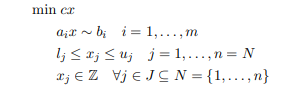
\includegraphics [scale = 0.7]{mip_scheme.png}
    \caption{ Formulazione MIP }
    \label{fig:mip}
\end{figure}\\
Si può notare che, conseguentemente all’inserimento dei vincoli di interezza delle variabili,
non possa essere usato direttamente un rilassamento lineare per la soluzione di questo
problema; il rilassamento ottenuto potrebbe contenere variabili con valore frazionario
quando nel problema di partenza le stesse variabili appartenevano al dominio degli interi.
Per la risoluzione di questo tipo di problemi viene generalmente impiegato un algoritmo 
chiamato “branch and cut”, una versione migliorata dell’algoritmo branch and bound.

\section{L'algoritmo b\&b}
Il b\&b è lo strumento più importante per la soluzione di problemi MIP. Il primo passo del 
metodo consiste nel rilassamento lineare del problema P di partenza e nelle considerazioni
successive: se il rilassamento è impossibile allora anche il problema P è impossibile, 
se si è trovata una soluzione al rilassamento e questa è ammissibile per P allora la 
soluzione è ottima per P, se la soluzione esiste ma non è intera allora il valore f(\textbf{x\textup{*}}) 
sarà un lower bound del problema di partenza.
Nell’ultimo caso (il più frequente) la soluzione del rilassamento \[\textbf{x}\textup{*} = 
(x \textsubscript{1} \textup{*}, …, x\textsubscript{n} \textup{*})\] non rispetta alcuni 
vincoli di interezza delle variabili di P ed è quindi necessaria la fase di branching.
In questa fase viene considerata una strategia di branching per dividere il problema P 
in sottoproblemi che vadano a risolvere le conflittualità dovute ai vincoli di interezza 
delle variabili del problema di partenza. Verrà poi eseguita di nuovo una 
fase di bound per ogni nuovo nodo e così via.
L’albero che si delinea può essere ridotto con una fase di pruning facendo delle 
considerazioni:
\begin{itemize}
    \item Se il rilassamento del nodo è impossibile posso scartare il nodo poichè
        il problema rilassato ha più gradi di libertà del problema non rilassato e
        quindi se il problema rilassato è impossibile anche il problema non rilassato, che
        non è altro quindi che una restrizione del rilassamento, è impossibile;
    \item Se il rilassamento mi ritorna una soluzione ammissibile per P ossia 
    \[\textbf{x*} \epsilon F(P)\] allora:
        \begin{itemize}
            \item Se è la prima soluzione che trovo salvo il suo valore (incumbent);
            \item Se il valore che trovo è inferiore al valore dell’incumbent già 
                trovato allora sostituisco l’incumbent con nuovo valore e salvo la 
                soluzione;
            \item Se il valore è inferiore all'incumbent già presente non posso dedurre nulla,
                continuo l'esplorazione dell'albero;
        \end{itemize}
    \item Se il rilassamento ritorna una soluzione non ammissibile per P ma il valore 
        dell’incumbent è inferiore al valore del rilassamento in questo nodo allora posso
        scartare il nodo. Il nodo attuale infatti ha valore del rilassamento superione ad un
        candidato ad essere soluzione ottima di P, quindi i nodi successivi non porterebbero 
        alcun miglioramento alla f.o. essendo questi una restrizione del problema a questo nodo. 
\end{itemize}
Quando ho finito di esplorare tutti i nodi il valore dell’incumbent (se presente) sarà la soluzione ottima.
\section{b\&c}
Il procedimento è analogo a b\&b con l’aggiunta nella fase di bound di piani di taglio. Questi
piani di taglio sono delle disgiunzioni lineari che riducono lo spazio delle soluzioni
togliendo dal pool alcune soluzioni non ammissibili per il problema di partenza. In modo
geometrico prendendo come riferimento un generico politopo posso descrivere un piano di
taglio come segue:\\
\begin{figure}[ht]
    \centering
    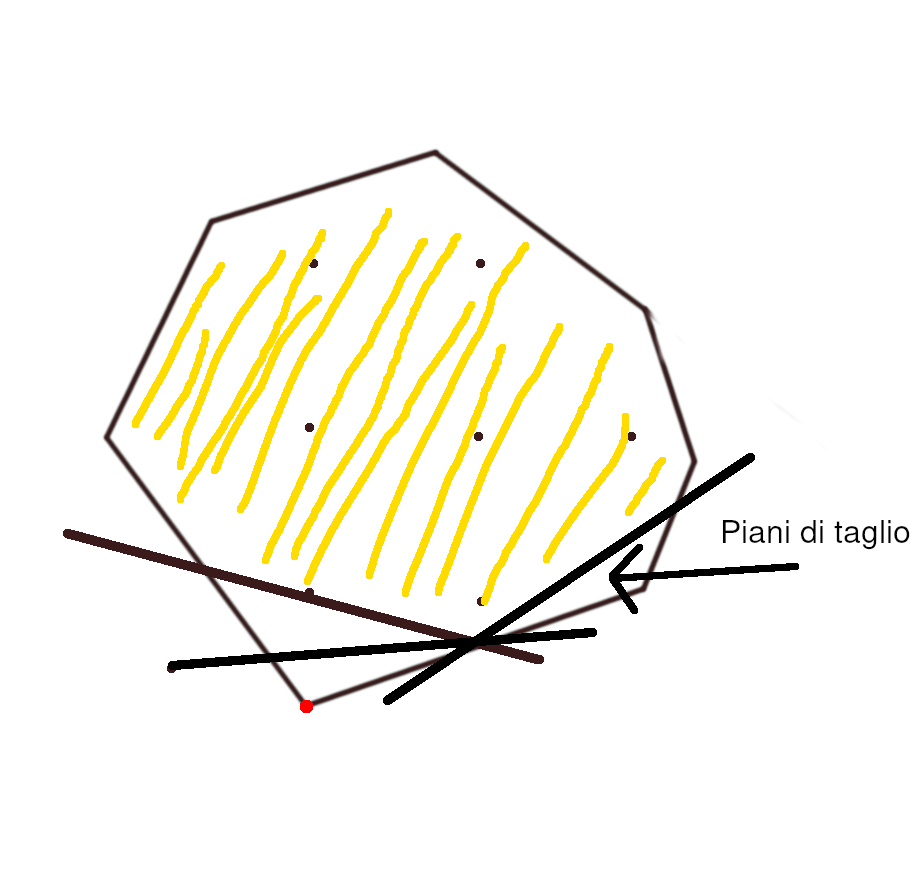
\includegraphics [scale = 0.7]{cutting_planes.png}
    \caption{Piani di taglio. }
    \label{fig:cuts}
\end{figure}\\
Trovare dei piani di taglio efficaci riduce notevolmente il tempo di esecuzione e anche se non fosse 
possibile trovarne al nodo attuale l'algoritmo continuerebbe in stile b\&b.
\section{Strong Branching}
Una delle strategie di branching applicate negli algoritmi b\&b e b\&c è lo strong branching:
questa strategia consiste nel prendere le variabili con vincoli di interezza non soddisfatti
nel rilassamento del nodo attuale, eseguire per ogni variabile il rilassamento lineare
ponendo prima come Upper Bound \[UB = \lfloor x \textsubscript{j} \textup{*} \rfloor\] e poi come Lower Bound 
\[LB = \lceil x \textsubscript{j} \textup{*} \rceil\] e vedere quale di queste variabili frazionarie
fornisce una separazione più importante. La separazione più forte sarà quella che verrà 
preferita nella creazione dei prossimi nodi.
\section{Clique Constraints}
I vincoli presi come candidati ad essere un miglioramento dello strong branching sono i 
vincoli di clique. Posso esprimere un vincolo di clique come segue:

\begin{center}
    $ 0 \leq \sum\limits_{i \epsilon I}^{} x\textsubscript{i} \leq 1 $  oppure $ \sum\limits_{i \epsilon I}^{} x\textsubscript{i} = 1 $

    $in\:cui\:I\:\acute{e}\:un\:sottoinsieme\:dell'enumerazione\:delle$

    $\:variabili\:booleane\:del\:problema$\linebreak
\end{center}

Questi vincoli possono essere rappresentati come una cricca (clique in inglese) ossia un grafo 
non orientato \[G = (E, V)\] in cui per ogni coppia di vertici \[x,y\:\epsilon\:V\] esiste 
un arco \[e\:\epsilon\:E\] che li congiunge.\pagebreak
\begin{figure}[ht]
    \centering
    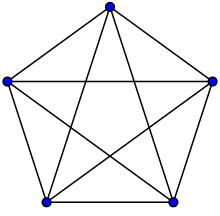
\includegraphics [scale = 0.5]{cricca.png}
    \caption{Rappresentazione grafica di una Cricca. }
    \label{fig:cricca}
\end{figure}\\
Si può notare che questo vincolo è molto sbilanciato quando si parla di decidere se impostare
variabile a 0 o a 1: la scelta di mettere una variabile a 1 nel vincolo limita tutte le 
altre variabili (avranno valore 0) mentre se la stessa variabile viene assegnata a 0 le rimanenti variabili 
non sono univocamente definite. Su questa osservazione si basa la tesi.

\chapter{Strong Branching on Clique Constraint}
\section{L'idea}
I vincoli di clique, come visto nel capitolo precedente, hanno un marcato sbilanciamento quando si 
tratta di fissare una variabile; da questa considerazione è scaturita questa raccolta dati, 
che si prefigge il compito di raccogliere del materiale per una possibile futura implementazione di una 
strategia di branching sui vincoli di clique. La SBCC si propone di testare, come nel semplice Strong Branching,
quale dei vincoli di clique del problema porta un miglioramento nella f.o.. 
L'obiettivo rimane comunque quello di creare una separazione più forte di quella data dal singolo Strong Branching 
nel tentativo portare il valore della f.o. il più vicino possibile al valore dell'incumbent e quindi dimostrare
che la soluzione per ora migliore sia quella ottima.
L'approccio di utilizzare il miglior risultato conosciuto al momento è naturalmente un approccio
euristico alla pari della strategia Strong Branching.
La strategia va a creare molti più nodi per ogni separazione rispetto a S.B. ma si può presumere che 
molti di questi nodi non verranno mai esporati e che saranno eliminati nella fase di pruning; oltre a ciò
lo Strong Branching fissa solo una variabile per ogni iterazione mentre la nuova strategia andrebbe a fissare 
il valore a tutte le variabili del vincolo. \\
Si può osservare inoltre che la strategia proposta non esclude alcuna soluzione ammissibile per il
problema proprio per la struttura del vincolo di clique.

\section{La raccolta dati}
Per effettuare delle considerazioni sulla effettiva efficacia della strategia è stata effettuata 
una raccolta dati prendendo in esame i problemi di programmazione intera-mista(MIP) presenti
nella libreria Miplib2003. L’algoritmo, scritto in C++ sfruttando le API del risolutore 
commerciale CPLEX 12.10 di IBM, si è concentrato inizialmente in un esame preliminare del 
problema P in ingresso in cui viene verificata la presenza di vincoli di clique tra i vincoli di P. 
Successivamente sono stati eseguiti per ogni variabile binaria il rilassamento in altro ed in basso 
(UB  = 0 e LB = 1) e sono stati salvati i valori della funzione obiettivo. \\
Sono state considerate solo le variabili binarie presenti nei vincoli di clique: un confronto globale
su tutte le variabili intere sarebbe stato molto costoso computazionalmente e non avrebbe messo bene 
in luce la convenienza dell'utilizzare la SBCC rispetto al semplice SB nello stesso campione di variabili.\\
Alla fine sono stati raggruppati i risultati per ogni vincolo di clique e salvati in un file di testo. 
La prima parte dell’algoritmo è stata fondamentale per scartare in partenza dei MIP senza 
questi vincoli e quindi evitare elaborazioni inutili.
\clearpage
\pagebreak 
Di seguito un resoconto sui problemi considerati:

\begin{center}
    \begin{tabular}{|c|c|c|c|c|c|}
        \hline
        Problema&Considerato&Scartato&Problema&Considerato&Scartato \\
        \hline
        10teams & X &  & momentum2 & X & \\
        \hline
        a1c1s1 & & X & momentum3 & X & \\
        \hline
        aflow30a & X & & msc98-ip & X & \\
        \hline
        aflow40b & X & & mzzv11 & & X \\
        \hline
        air04 & X & & mzzv42z & & X \\
        \hline
        air05 & X & & net12 & & X \\
        \hline
        arki001 & & X & noswot & & X \\
        \hline
        atlanta-ip & X & & nsand-ipx & & X \\ 
        \hline
        cap6000 & X & & nw04 & X & \\ 
        \hline
        dano3mip & X & & opt1217 & X & \\
        \hline
        disctom & X & & p2756 & & X \\
        \hline 
        ds & X & & pk1 & & X \\
        \hline
        fast0507 & & X & pp08a & & X \\
        \hline
        fiber & X & & pp08aCUTS & & X \\
        \hline
        fixnet6 & & X & protfold & X & \\
        \hline
        gesa2 & & X & qiu & & X \\
        \hline
        gesa2-o & & X & rd-rplusc-21 & X & \\
        \hline
        glass4 & X & & roll300 & & X \\
        \hline
        harp2 & X & & rout & & X \\
        \hline
        liu & & X & set1ch & & X \\
        \hline
        manna81 & & X & seymour & & X \\
        \hline
        markshare1 & & X & sp97ar & &X \\
        \hline
        markshare2 & & X & stp3d & X & \\
        \hline
        mas74 & & X & swath & X & \\
        \hline
        mas76 & & X & t1717 & X & \\
        \hline
        misc07 & X & & timtab1 & & X \\
        \hline
        mkc & & X & timtab2 & & X \\
        \hline
        mod011 & X & &tr12-30 & & X \\
        \hline
        momentum1 & X & & vpm2 & & X \\
        \hline
    \end{tabular}
\end{center}

Oltre a verificare la presenza o meno di vincoli di clique in questa prima parte del programma
vengono salvate le posizioni delle variabili binarie e dei vincoli di clique essendo dati 
utili per la successiva elaborazione.\\ Nella seconda fase vengono risolti 2 rilassamenti 
per ogni variabile binaria (impostando prima la variabile a 0 e poi a 1). Per ogni vincolo 
di <= inoltre viene calcolato il valore del rilassamento con tutte le variabili a 0.\\I valori 
ottenuti dai rilassamenti saranno poi il punto cardine nell'analisi dell'efficacia o meno
della strategia di branching ipotizzata. \\
\begin{figure}[ht]
    \centering
    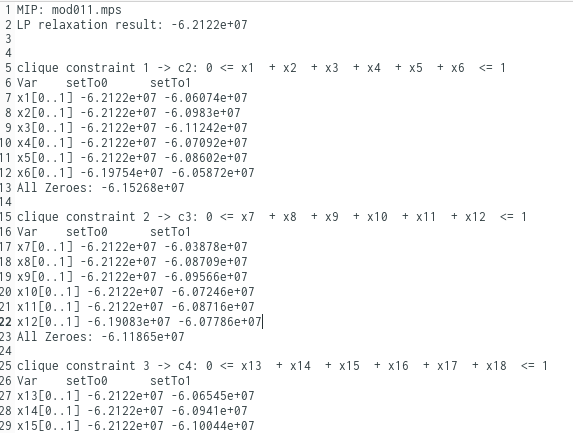
\includegraphics [scale = 0.5]{output_example.png}
    \caption{Esempio file di output.}
    \label{fig:output}
\end{figure}

\subsection{Miplib2003}
I problemi da cui sono state estratte le informazioni sono contenuti nella libreria Miplib2003.
La libreria si configura come una collezione di 60 problemi MIP di natura varia ideali per avrebbe
un insieme eterogeneo di istanze. La scelta di una libreria datata (i problemi della libreria 
sono stati formulati dal 1999 al 2003) è stata effettuata consapevolmente data la necessità di avere 
istanze già risolte (in gran parte) e per la presenza di problemi di piccola taglia utili per fare 
delle osservazioni dettagliate.

\section{Software utilizzati}
Per raccogliere le informazioni dalla libreria Miplib2003 è stato utilizzato il risolutore 
commerciale CPLEX di IBM. Il programma si distingue in questo ramo 
dell'informatica per le buone performance della sua implementazione dell'algoritmo del 
simplesso e per le molte features messe a disposizione all'utente finale.\\
Il programma che è stato implementato per la raccolta dati è stato scritto in C++ utilizzando 
le API del ramo Concert di CPLEX. Queste API, anche se non molto intuitive,
si sono dimostrate efficaci per l'implementazione del codice, permettendo all'utente di 
modificare ed esplorare facilmente il problema di partenza. Per le istanze più onerose 
computazionalmente è stata fondamentale la possibilità di iterare le variabili presenti nel
vincolo di clique senza dover risolvere tutti i rilassamenti di tutte le variabili booleane 
(il che avrebbe fatto aumentare esponenzialmente il tempo per la raccolta dati).\\\\

Per l'elaborazione dei dati sono stati utilizzati i runner appartenenti al Cluster del Dipartimento di Ingegneria 
dell'Informazione tramite il sistema di somministrazione dei job SLURM: 
processare un numero così elevato di rilassamenti lineari non risulta possibile con soluzioni 
economiche e questi strumenti messi a disposizione dal DEI sono stati fondamentali per 
la riuscita di questo progetto.
\\
Per l'analisi dei dati è stato utilizzato il linguaggio di programmazione Python con il supporto delle 
librerie Numpy e MatplotLib.

\chapter{Risultati}
Di seguito alcune considerazioni sui dati ottenuti. Essendo questa un'analisi preliminare della strategia
non sono stati raccolti i risultati a livello prestazionale ma semplicemente dei $numeri$ utili a capire se 
questa strategia ha delle possibilità applicative.

\section{Considerazioni sui dati ottenuti}
Data la grande quantità di dati ottenuti risulta necessario aggregare alcuni risultati. Il primo indicatore
utilizzato per verificare il potenziale della SBCC è il seguente: per ogni vincolo di clique 
$j\:\:\epsilon\:\:Cliques$ è stato calcolato un valore
\[ s\textsubscript{j} = \sqrt[n]{\prod_{i=1}^{n\textsubscript{j}} (R(x\textsubscript{i}=1)-R\textsubscript{ref}) }\] 
in cui $R(x\textsubscript{i})$ è il valore del rilassamento fissando a 1 la variabile $x\textsubscript{i}$
del vincolo, $R\textsubscript{ref}$ è il valore del rilassamento del problema iniziale e$n\textsubscript{j}$ è il 
numero di variabili comprese nel vincolo di clique. Nel caso il vincolo di clique sia di <= nella 
produttoria verrà inserito un ulteriore termine $(R(x\textsubscript{1}=0, .., x\textsubscript{n}=0)- R\textsubscript{ref})$.
Per confronto ad ogni variabile binaria $k\:\epsilon\:Binaries$ coinvolta in almeno un vincolo di clique è stato assegnato uno score
\[ b\textsubscript{k} = \sqrt{(R(x\textsubscript{k}=0)-R\textsubscript{ref})*(R(x\textsubscript{k}=1)-R\textsubscript{ref})}\] 
Si può notare che nel caso uno dei valori nella produttoria è 0 allora lo score sarà 0, per ovviare a ciò
è stato considerato il valore 0.01 al posto di 0.\\
Per ogni problema è stato raccolto il migliore $s\textsubscript{j}$ e $b\textsubscript{k}$ ed è stato fatto il rapporto
tra i due valori. Se questo è > 1 allora almeno una clique del problema ha creato una separazione migliore del semplice SB
sulle variabili binarie.\\\pagebreak
\\Di seguito il grafico ottenuto[Figura 3.1]:\\

\begin{figure}[ht]
    \centering
    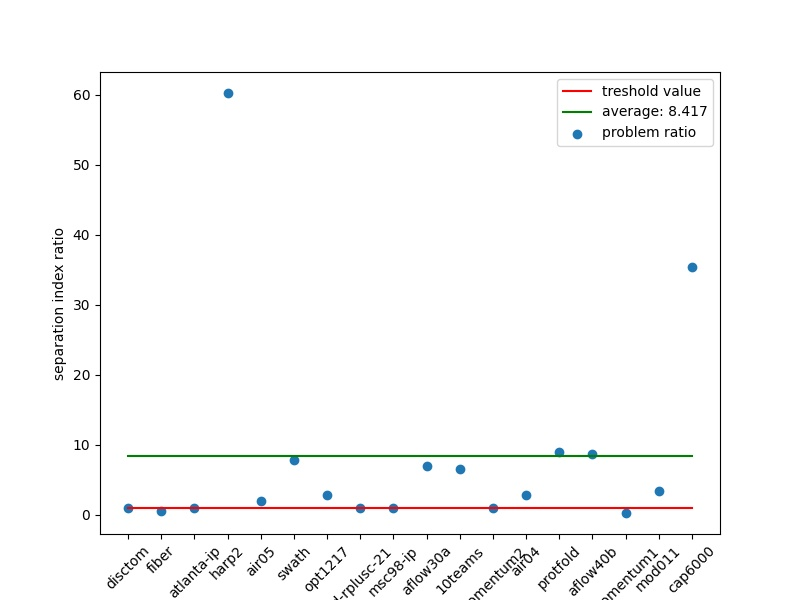
\includegraphics [scale = 0.7]{chart_agg}
    \caption{Problem ratio}
    \label{fig:ratio}
\end{figure}
Si può osservare che in molti dei problemi la separazione che va a crearsi è migliore della miglior separazione 
tramite Strong Branching delle variabili coinvolte nei vincoli. \\
I risultati ottenuti, come si può vedere, sono promettenti: in media una separazione creata tramite clique risulta
8 volte più forte di una separazione traqmite SB. \pagebreak
\section{Mod011.mps}
A campione è stato analizzato il problema mod011.mps. La taglia dell'istanza considerata è relativamente piccola
e non necessita un'aggregazione di dati per essere analizzata. Dal file di output creato è stato realizzato un grafico
in cui ogni vincolo di clique del problema è stato messo in confronto con la migliore separazione ottenuta dalle variabili
contenute nel vincolo stesso tramite SB[Figura 3.2]. L'indice considerato è lo stesso della sezione precedente.\\
\begin{figure}[ht]
    \centering
    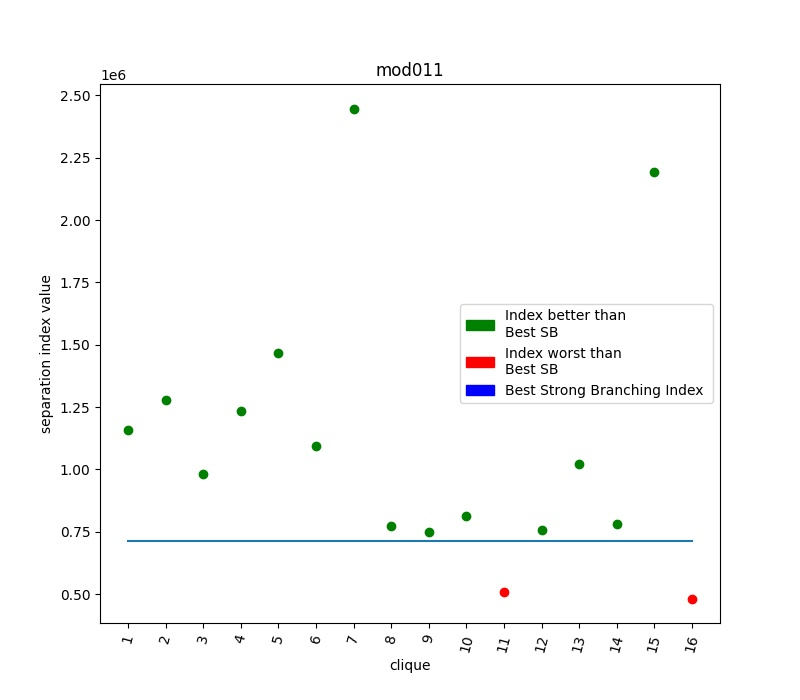
\includegraphics [scale = 0.7]{chart_exp1_mod011}
    \caption{Mod011 chart}
    \label{fig:mod011}
\end{figure}\\
Si può notare che in relazione alle variabili presenti nel vincolo tutte le separazioni tramite clique risultano più forti 
e che rispetto alla migliore separazione solo 2 vincoli su 16 risultano inferiori.
\\
\chapter{Conclusioni}
\addcontentsline{toc}{chapter}{\bibname}
\renewcommand{\bibname}{Bibliografia/Sitografia}
\begin{thebibliography}{100}
    \bibitem{} Lezioni di Ricerca Operativa, M. Fischetti, 2018;
    \bibitem{} Constraint Integer Programming, T. Achterberg, 2007;
    \bibitem{} Cplex User Manual: \\ 
    $https://www.ibm.com/support/knowledgecenter/SSSA5P_12.7.1/
    \\ilog.odms.studio.help/pdf/usrcplex.pdf$
\end{thebibliography}



\end{document}